\section{Theorie}
\label{sec:Theorie}

% zielsetzung
In diesem Versuch werden verschieden elektrische Bauteile in Brückenschaltungen
eingesetz, um deren (komplexen) Widerstände zu bestimmen.

Dabei wird hier mit der Nullmethode gearbeitet, d.h. dass durch variable Bauteile
die Brückenspannung zum verschwinden gebracht wird.

Zuletzt soll noch der Klirrfaktor des benutzten Funktionenerzeugers bestimmt werden.

\subsection{Kirchoffschen Gesetze}
\label{sec:kirchhoff}
Zur Berechnung vom Stromfluss in Schaltungen werden zwei Gesetze, die
kirchhoffschen Gesetze, verwendet:
\begin{enumerate}
	\item Die \textbf{Knotenregel} besagt, dass an jedem Punkt in einem Stromkreis
		die Summe aller Ströme (wobei Eingangsströme mit $\mathbf{I} > 0$ und
		Ausgangsströme mit $\mathbf{I} < 0$ betrachtet werden) verschwindet:
		\begin{equation}
			\sum_k \mathbf{I}_k = 0.
			\label{eqn:knotenregel}
		\end{equation}
		\begin{figure}[H]
			\centering
			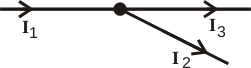
\includegraphics[width=0.4\textwidth]{bilder/knotenregel.png}
			\caption{Darstellung eines ``Knotens`` in einem Stromkreis}
			\label{fig:knotenregel}
		\end{figure}
	\item Nach der \textbf{Maschenregel} ist die Summe der Potentialdifferenzen
		in einem geschlossenen Stromkreis (``Masche``) 0:
		\begin{equation}
			\sum_k U_k = \sum_k \mathbf{I}_k R_k= 0
			\label{eqn:maschenregel}
		\end{equation}
		\begin{figure}[H]
			\centering
			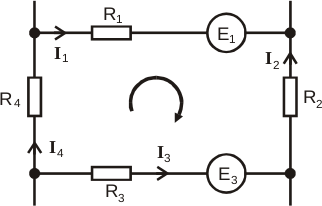
\includegraphics[width=0.5\textwidth]{bilder/maschenregel.png}
			\caption{Darstellung einer Masche in einem Leiternetzwerk}
			\label{fig:maschenregel}
		\end{figure}
\end{enumerate}

\subsection{Berechnung der Brückenspannung und Herleitung der 
Abgleichbedingung}
\label{sec:abgleichbedingung}

In einer Brückenschaltung werden die Stromflüsse in zwei parallelen (jedoch in ihren
Bauteilen nicht unbedingt gleichen) Stromleitern zwischen zwei Punkten (in 
\autoref{fig:prinzipielle-brueckenschaltung} als A und B bezeichnet) die Potentialdifferenz 
betrachtet.
Diese Potentialdifferenz wird im Allgemeinen als Brückenspannung bezeichnet.

\begin{figure}[H]
	\centering
	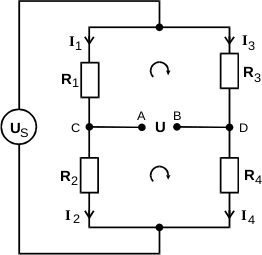
\includegraphics[width=0.5\textwidth]{bilder/prinzipielle-brueckenschaltung.png}
	\caption{Prinzipielle Brückenschaltung}
	\label{fig:prinzipielle-brueckenschaltung}
\end{figure}

Mit dem ersten kirchhoffschen Gesetz lassen sich dann für $U=0$ die Bedingungen für
die parallelen Ströme herleiten:
\begin{equation}
	\mathbf{I}_1 = \mathbf{I}_2
	\quad \text{und} \quad
	\mathbf{I}_3 = \mathbf{I}_4.
	\label{eqn:brueckenschaltung-stroeme}
\end{equation}

Das zweite Kirchhoffsche Gesetz gibt Auskunft über die Spannungen:
\begin{equation}
	U = - R_1 \mathbf{I}_1 + R_3 \mathbf{I}_3
	%\quad
	\text{ und }
	%\quad
	-U = -R_2 \mathbf{I}_2 + R_4 \mathbf{I}_4.
	\label{eqn:allgemein-kirchhoff2}
\end{equation}
In \autoref{eqn:allgemein-kirchhoff2} können dank \autoref{eqn:brueckenschaltung-stroeme} 
$\mathbf{I}_2$ und $\mathbf{I}_4$ durch $\mathbf{I}_1$ bzw. $\mathbf{I}_3$ ersetzt werden.
\\
Gleichsetzen beider Ausdrücke liefert dann
\begin{equation}
	U = \frac{R_2 R_3 - R_1 R_4}{R_3 + R_4} \mathbf{I}_1.
	\label{eqn:ablgeich-abhaengig}
\end{equation}

Mit der Speisespannung
\begin{equation}
	U_S = \mathbf{I}_1 (R_1 + R_2)
	\label{eqn:speisespannung}
\end{equation}
lautet die Brückenspannung
\begin{equation}
	U = \frac{R_2 R_3 - R_1 R_4}{(R_3 + R_4)(R_1 + R_2)} U_S.
	\label{eqn:brueckenspannung-unabhaengig}
\end{equation}

Die Brückenspannung verschwindet wenn der Zähler im Bruch 0 ist, also
\begin{equation}
	R_1R_4 = R_2R_3.
	\label{eqn:prinzipielle-abgleichbedingung}
\end{equation}

Im Falle $U=0$ spricht man auch von einer abgeglichenen Brücke. Da die 
Abgleichbedingung nur von den Widerständen abhängt, kann damit ein unbekannter Widerstand
bestimmt werden. Die Genauigkeit von einer Messung hängt dann nur noch von der Genauigkeit
der bekannten Widerstände und davon, wie niedrig die Brückenspannung in ihrem Minimum ist
(da $U=0$ auch nur ein theoretisches Optimum ist).
Da die Brückenspannung proportional zur Speisespannung ist, sollte Letztere möglichst
groß gewählt werden.

\subsection{Verallgemeinerung auf komplexe Widerstände}
\label{sec:komplexe-widerstände}
Wenn die Brückenschaltung nicht nur Widerstände, sondern auch Kapazitäten und Induktivitäten
enthält, muss der Formalismus aus \autoref{sec:abgleichbedingung} auf diese verallgemeinert
werden. Dazu bietet sich die Darstellung als komplexer Widerstand
\begin{equation}
	Z = X + jY
	\label{eqn:komplexer-widerstand}
\end{equation}
an, wobei X den leistungsverbrauchenden Wirkwiderstand und Y den Blindwiderstand darstellt.

Die Abgleichbedingung aus \autoref{eqn:prinzipielle-abgleichbedingung} muss dann als komplexe
Gleichung interpretiert werden, d.h. dass Imaginär- und Realteil auf beiden Seiten gleich sein
müssen. Da aus der Darstellung als komplexer Widerstand zwei Unbekannte ($X$ und $Y$) resultieren,
folgen damit auch zwei Gleichungen:
\begin{equation}
	X_1X_4 - Y_1Y_4 = X_2X_3 - Y_2Y_3 
	\quad \text{und} \quad
	X_1Y_4 - X_4Y_1 = X_2Y_3 - X_3Y_2.
	\label{eqn:komplexe-abgleichbedingung}
\end{equation}
Elektrotechnisch bedeutet dies, dass sowohl Betrag, als auch Phase des Wechselstroms verschwinden
müssen. Aus den zwei Freiheitsgraden folgt auch, dass an der Brückenschaltung zwei voneinander
unabhängige Stellglieder existieren müssen.

\subsection{Verwendete Widerstände}
\label{seq:widerstände}
In diesem Versuch werden ausschließlich Ohm'sche Widerstände benutzt. Von Interesse sind dabei
die Intuktivität (Zeichen: L), die Kapazitäten (C) und die gewöhnlichen, nicht-komplexen 
Widerstände R.

Die Impedanzen im komplexen sind dabei
\begin{align}
	Z_R &= R, \\
	Z_L &= j\omega L, \\
	Z_C &= -\frac{j}{\omega} L.
	\label{eqn:impedanzen}
\end{align}
Dabei sollte beachtet werden, dass diese auch von der Kreisfrequenz des Wechselstroms $\omega$ 
abhängig sein können. 

\subsection{Beschreibung der verwendeten Brückenschaltungen}
\label{sec:spezielle-Schaltungen}

Im Nachfolgenden Abschnitt wird auf einige spezielle Brückenschaltungen eingegangen und mithilfe von
\autoref{eqn:prinzipielle-abgleichbedingung} und \autoref{eqn:komplexe-abgleichbedingung} 
eine Formel für das unbekannte Bauteil hergeleitet.

\subsubsection{Wheatstonesche Brücke}
\label{sec:theorie-wheatstone}
In der Wheatstoneschen Brücke sind alle $R_i$ ohmsche Widerstände, wobei hier $R_1$ ein unbekannter
Widerstand ist, die Anderen sind bekannt.

\begin{figure}[H]
	\centering
	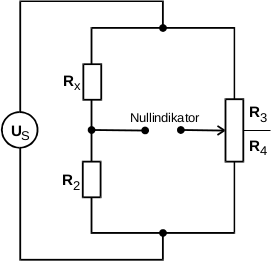
\includegraphics[width=0.4\textwidth]{bilder/wheatstone.png}
	\caption{Schaltplan der Wheatstoneschen Brückenschaltung}
	\label{fig:wheatstone-bruecke}
\end{figure}

Mit \autoref{eqn:prinzipielle-abgleichbedingung} lautet dann der unbekannte Widerstand
\begin{equation}
	R_x = R_2 \frac{R_3}{R_4}.
	\label{eqn:wheatstone-rx}
\end{equation}

\subsubsection{Kapazitätsmessbrücke}
\label{sec:theorie-kapazitaetsmessbruecke}

Wie der Name andeutet, können mit dieser Brückenschaltung die Kennzahlen eines Kondensators bestimmt werden.
Ein realer Kondensator besitzt allerdings nicht nur den komplexen Anteil wie in \autoref{eqn:impedanzen},
sondern hat auch dielekterische Verluste.

Daher benutzt man ein Ersatzschaltbild mit einem Widerstand $R$.
\begin{figure}[H]
	\centering
	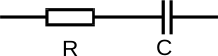
\includegraphics[width=0.3\textwidth]{bilder/ersatz-kapazitaet.png}
	\caption{Ersatzschaltbild eines realen Kondensators.}
	\label{fig:ersatz-kondensator}
\end{figure}
Der reale Widerstand lautet somit
\begin{equation}
	Z_{C_\text{real}} = R - \frac{j}{\omega C}.
	\label{eqn:realer-wderstand-kondensator}
\end{equation}

Da jetzt für den unbekannten Kondensator $R_{C_\text{real}}$ zwei unbekannte vorliegen ($R$ und $C$), muss 
auch ein weiterer Freiheitsgrad zur Abstimmvorrichtung hinzugefügt werden.

In diesem Versuchsaufbau (siehe \autoref{fig:kapazitaetsbruecke}) wird dieser durch einen Veränderlichen $R_2$
realisiert.
\begin{figure}[H]
	\centering
	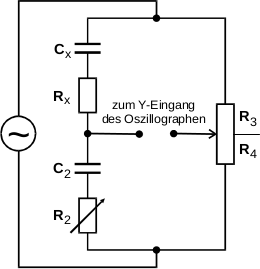
\includegraphics[width=0.4\textwidth]{bilder/kapazitaetsbruecke.png}
	\caption{Schaltplan zur Kapazitätsmessbrücke.}
	\label{fig:kapazitaetsbruecke}
\end{figure}

Die Abgleichbedingung liefert dann
\begin{equation}
	R_x = R_2 \frac{R_3}{R_4}
	\qquad
	C_x = C_2 \frac{R_4}{R_3}
	\label{eqn:values-kapazitaeten}
\end{equation}

\subsubsection{Induktivitätsmessbrücke}
\label{sec:theorie-induktivitätsmessbrücke}

Wie eben schon für Kondensatoren, müssen hier auch für Spulen einige Vorüberlegungen getroffen werden.
Diese sind auch verlustbehaftet, weswegen auch hier ein Ersatzschaltbild mit einem Widerstand zum Einsatz kommt.
Die Impedanz lautet dann
\begin{equation}
	Z_{L_\text{real}} = R + j \omega L.
	\label{eqn:reale-induktivitaet}
\end{equation}

Der Aufbau der Induktivitätsmessbrücke besitzt erfolgt analog zu der Kapazitätsmessbrücke:
\begin{figure}[H]
	\centering
	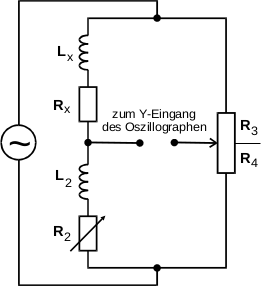
\includegraphics[width=0.4\textwidth]{bilder/induktivitaetsbruecke.png}
	\caption{Schaltplan zur Induktivitätsmessbrücke.}
	\label{fig:induktivitaetsbruecke}
\end{figure}

Die Kennziffern der unbekannten Spule folgen dann aus \autoref{eqn:komplexe-abgleichbedingung}:
\begin{equation}
	R_x = R_2 \frac{R_3}{R_4}
	\qquad
	L_x = L_2 \frac{R_3}{R_4}.
	\label{eqn:values-induktivitaetsbruecke}
\end{equation}


\subsubsection{Maxwell-Brücke}
\label{sec:theorie-maxwell-bruecke}

Eine Alternative zu der in \autoref{sec:theorie-induktivitätsmessbrücke} diskutierten Methode zur
Bestimmung unbekannter Induktivitäten ist die Maxwell-Brücke, die Schaltung ist in 
\autoref{fig:maxwell-schaltplan} zu sehen.
\begin{figure}[H]
	\centering
	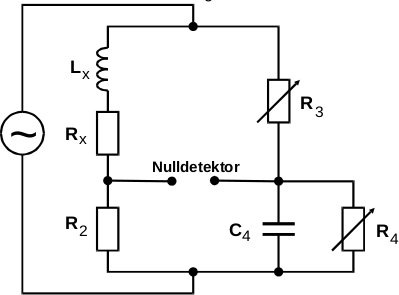
\includegraphics[width=0.5\textwidth]{bilder/maxwellbruecke.png}
	\caption{Schaltplan zur Maxwell-Brücke.}
	\label{fig:maxwell-schaltplan}
\end{figure}

Der Unterschied zur Induktivitätsbrücke besteht dadrin, dass $R_2$ konstant gehalten wird und keine 
Induktivität enthält. Der zweite Freihatsgrad im System wird durch den parallel liegenden, nun
variablen $R_4$ mit einem parallel geschalteten Kondensator $C_4$ realisiert.

Aus \autoref{eqn:komplexe-abgleichbedingung} folgen dann die Gleichungen
\begin{equation}
	R_x R_4 + \omega^2 R_4^2 C_4 L_x = R_2 R_3 \left(1 + \omega^2 C_4^2 R_4^2 \right)
	\label{eqn:maxwell-gleichung1}
\end{equation}
und
\begin{equation}
	-\omega R_x R_4^2 C_4 = 0.
	\label{eqn:maxwell-gleichung2}
\end{equation}
Diese liefern die unbekannten Größen
\begin{equation}
	R_x = \frac{R_2 R_3}{R_4}
	\qquad
	L_x = R_2 R_3 R_4.
	\label{eqn:kenngroessen-maxwell}
\end{equation}

\subsubsection{Wien-Robinson-Brücke}
\label{sec:theorie-wien-robinson-bruecke}
Zuletzt wird hier jetzt die Wien-Robinson-Brücke beschrieben. Diese unterscheidet sich von den 
bisher genannten Schaltungen dadurch, dass die Ablgeichbedingung auch von der Frequenz des Wechselstroms $\omega$
abhängt.
\begin{figure}[H]
	\centering
	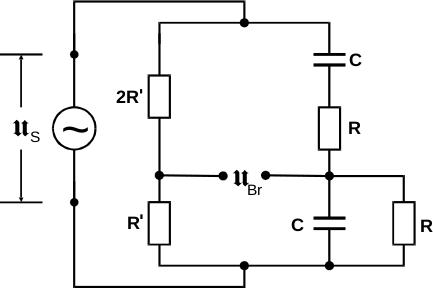
\includegraphics[width=0.5\textwidth]{bilder/wien-robinson.png}
	\caption{Schaltplan zur Wien-Robinson-Brücke.}
	\label{fig:wien-robinson-schaltplan}
\end{figure}

Die vier Brückenelemente besitzen damit die Widerstandsoperatoren
\begin{equation}
	Z_1 = 2R^\prime,
	\quad
	Z_2 = R^\prime,
	\quad
	%Z_3 = R + \frac{1}{j\omega C},
	Z_3 = \frac{j\omega RC + 1}{j \omega C}
	\quad
	\text{und }
	Z_4 = \frac{R}{1 + j\omega RC}.
\end{equation}

Damit folgt aus \autoref{eqn:komplexe-abgleichbedingung}
\begin{align}
	U_\text{Br} 
	&= \frac{
		\frac{2 R R^\prime}{1 + j\omega RC}
		- \frac{R^\prime + j \omega R^\prime RC}{j\omega C}
	}
	{3 R^\prime \left(\frac{j \omega RC +1}{j\omega C}
			+ \frac{R}{1 + j \omega RC}
		\right)
	}
	U_S
	\\
	&= \frac{\omega^2 R^2 C^2 - 1}
	{3 \left(1 - \omega^2 R^2C^2\right) + 9 j\omega RC}
	U_S.
\end{align}

Das Verhältnis zwischen Brückenspannung und Speisespannung lautet somit
\begin{equation}
	\left|\frac{U_\text{Br}}{U_S}\right|^2
	=
	\frac{\left(\omega^2R^2C^2 - 1 \right)^2}
	{9 \left\{ \left(1 - \omega^2R^2C^2\right)^2 + 9\omega^2R^2C^2 \right\}}.
	\label{eqn:verhaeltnis-wien-robinson}
\end{equation}

Offensichtlich verschwindet \autoref{eqn:verhaeltnis-wien-robinson} für
\begin{equation}
	\omega = \omega_0 = \frac{1}{RC}.
	\label{eqn:wien-robinson-w0}
\end{equation}
Eine einfachere Darstellung von \autoref{eqn:verhaeltnis-wien-robinson} ist möglich durch
das Frequenzverhältnis
\begin{equation}
	\Omega := \frac{\omega}{\omega_0},
	\label{eqn:wien-robinson-frequenz}
\end{equation}
das ergibt dann
\begin{equation}
	\left|\frac{U_\text{Br}}{U_S}\right|^2
	=
	\frac{1}{9}
	\frac{\left(\Omega^2 - 1\right)^2}{\left(1 - \Omega^2\right)^2 + 9\Omega^2}.
	\label{eqn:wien-robinson-abgleich-einfach}
\end{equation}

In \autoref{eqn:wien-robinson-abgleich-einfach} wird deutlich, dass es sich bei der 
Wien-Robinson-Brücke um einen elektronischen Filter handelt. Wechselströme mit der 
Kreisfrequenz $\omega$ werden entfernt und Frequenzen in der Nähe abgeschwächt.

\subsection{Bestimmung des Klirrfaktors}
\label{sec:klirrfaktor}

Der Klirrfaktor ist ein Indikator für die Qualität eines Funktionenerzeugers. Ein idealer 
Sinus-Generator erzeugt nur den Sinus zu der eingestellten Frequenz. Das ist beim realen 
Funktionen-Generator nicht der Fall; es entstehen Oberwellen.

Für die Bestimmung des Klirrfaktors wird die Wien-Robinson-Brücke aus 
\autoref{sec:theorie-wien-robinson-bruecke} benutzt. Mit ihr wird die Hauptwelle des 
Funktionenerzeugers rausgefiltert, sodass nur die Oberwellen zurückbleiben. Dann folgt der
Klirrfaktor
\begin{equation}
	k = \frac{\sqrt{U_2^2 + U_3^2 + \hdots}}{U_1}.
	\label{eqn:klirrfaktor}
\end{equation}
Dabei ist $U_1$ die Amplitude der Grundwelle und $U_n$ die der n-ten Oberwelle, welche dann die
Frequenz $n\omega_0$ besitzt.

Für diesen Versuch wird die Annahme 
\begin{equation}
	U_k = 0 \text{ für } k > 2
	\label{eqn:klirrfaktor-annahme}
\end{equation}
gemacht. Dann lautet folgt aus \autoref{eqn:wien-robinson-abgleich-einfach}
\begin{equation}
	U_2 = \frac{U_\text{Br}}{f(2)}
	\label{eqn:klirrfaktor-u2}
\end{equation}
Wobei $f(2)$ \autoref{eqn:wien-robinson-abgleich-einfach} bei $\Omega = 2$ ausgewertet ist.

